% Documentatie Herfstkamp project: Bouw van een audio-versterker
% Jules Hammenecker
% Vrije Universiteit Brussel - Dept. ELEC
% Augustus 2015

\title{Project Ingenieurswetenschappen: \\ Elektronisch ontwerp van de e-VUBOX}
\author{Vrije Universiteit Brussel}
\date{Versie 08.2015}

\documentclass{article}

	\usepackage[a4paper]{geometry}
	\usepackage[T1]{fontenc}
	\usepackage[dutch]{babel}
	\usepackage{amsmath}
	\usepackage{pdflscape}
		\newtheorem{DIY}{Doe-het-zelf}
	\usepackage{multicol}
\usepackage{enumerate}
	%%% FIGURES %%%

	\usepackage[pdftex]{graphicx}
	\usepackage{caption,subcaption}
	\usepackage{hyperref}
	\graphicspath{ {./figs/} }

\begin{document}
	\pagenumbering{roman}
	\maketitle

	\begin{figure}[htbp]
		\centering
		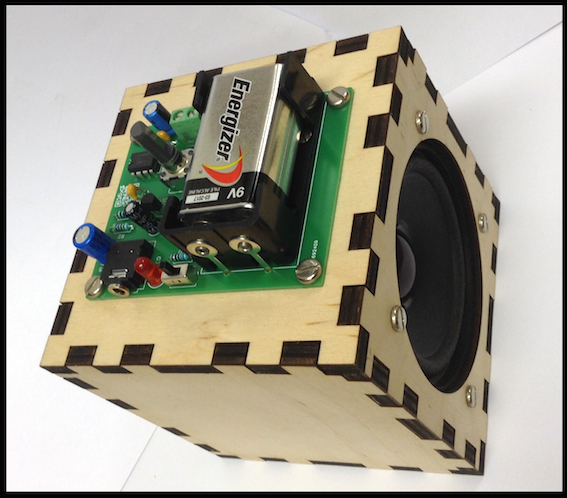
\includegraphics[width=0.6\textwidth]{foto.jpg}
		\caption{De prachtige e-VUBOX.}
		\label{fig:foto}
	\end{figure}

	\clearpage
	\tableofcontents
	\clearpage
\pagenumbering{arabic}
	\section{Doelstelling}
		Elektronische uitvindingen maken deel uit van de grote revoluties van onze tijd. Van eenvoudige rekenmachines tot de meest geavanceerde computers, spelconsoles, GPS-satellieten, zelfrijdende auto's, hersenimplantaten, pratende robots die duizenden objecten per seconde herkennen\ldots Die verbluffende uitvindingen worden dagelijks gemaakt en gebruikt.

		Al die fascinerende ontwikkelingen kunnen de ambitie geven om zelf elektronische wondermachines te maken, als je maar wist hoe die miraculeuse elektronica in elkaar zat. Goed nieuws, dit is het net doel van dit project. We gaan de mysteries van de elektronica ontfutselen door \textbf{een audio-versterker te bouwen, de e-VUBOX}. De e-VUBOX is een versterker, die energie pompt in de muziek van een muziekspeler. Dit is zodat er genoeg elektrisch vermogen is om het luid te kunnen afspelen door een luidspreker (figuur~\ref{fig:principe}). Je zal snel zien dat elektronische circuits niet (helemaal) magisch zijn!

		\begin{figure}[htbp]
			\centering
			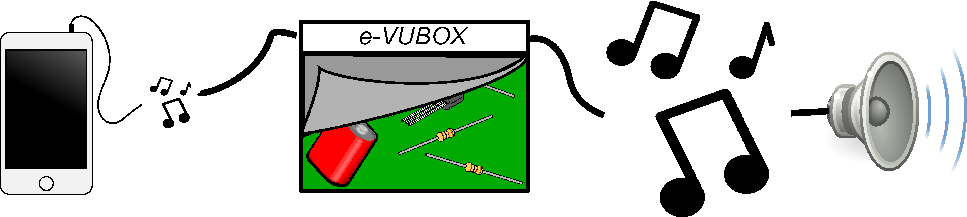
\includegraphics[scale=0.7]{principe}
			\caption{Principeschema van het project. We gaan muziek versterken, en gaan de mysteries van de elektronica binnen de e-VUBOX ontsluieren.}
			\label{fig:principe}
		\end{figure}

		Laten we beginnen met een overzicht van de wetten en vuistregels van de elektronica. Als je al een basis hebt in de elektronica, mag je onmiddellijk beginnen met hoofdstuk \ref{sec:bouwstenen}.
		\begin{DIY}
			Waarom is een versterker nuttig? Wat zou je nog kunnen aansluiten aan de ingang van een versterker?
		\end{DIY}
	\section{Elektronica: componenten en netwerken}

		Als elektronische ingenieur ga je nuttige elektronische netwerken maken door componenten op een slimme manier te schakelen. De schematische voorstelling van zo'n elektronische componenten en een netwerk zijn te vinden in Figuur \ref{fig:component_en_schakeling}. In de elektronica zijn er twee grootheden die we graag in het oog houden:

		\begin{enumerate}
			\item de \textbf{spanning} (symbool: $V$, $U$ of soms $E$) is het verschil in potenti\"ele elektrische energie tussen twee punten. Spanning wordt ook \emph{voltage} genoemd. De eenheid van spanning is de \emph{Volt}. Er is 1 Joule energie nodig om 1 Coulomb lading te verplaatsen door een spanningsval van 1 Volt. (De Coulomb is de eenheid van elektrische lading).

			\item de \textbf{stroom} (symbool: $I$) is de hoeveelheid lading per tijdseenheid dat vloeit door een punt. De eenheid van stroom is de Amp\`ere. Een stroom van 1 Amp\`ere is gelijk aan 1 Coulomb per seconde dat vloeit door een punt.
		\end{enumerate}

		Pas op: spreek altijd van een spanning \emph{tussen} twee punten in een netwerk. Spreek ook van een stroom \emph{door} een punt of een component. Zoiets zeggen als ``de spanning door een weerstand...'' is pure nonsens.

		Stromen en spanning kunnen constant zijn over de tijd, we spreken dan van DC (Direct Current). Als ze veranderen met de tijd, spreken we van AC (Alternating Current).
		\begin{DIY}
			Er is tussen twee punten van een netwerk een spanning V:

			\begin{align*}
			    V(t)  = 3~V + 1~V \cdot sin(2\pi \cdot 10~Hz \cdot t)
			\end{align*}
			Welke gedeelte van de spanning is DC, welk gedeelte is AC?
		\end{DIY}

		Stroom en spanning kunnen samenwerken om energie te leveren. We spreken dan van het elektrisch vermogen (symbool P, eenheid Watt). Het elektrisch vermogen dat een component verbruikt is het product van de stroom en de spanning:
		\begin{align}
		     P = V \cdot I
		     \label{eq:vermogen}
		 \end{align} 

		Elektrisch vermogen kan bvb. gebruikt worden door een led voor licht, door een luidspreker voor geluid of door een weerstand voor warmte.

		\begin{figure}[hbtp]
			\centering
			\begin{subfigure}[b]{0.4\linewidth}
				\centering
				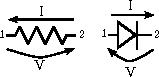
\includegraphics{componenten}
				\caption{Elektronische componenten: een weerstand links en een diode rechts. Men spreekt van de spanning $V$ \textbf{over} de pinnen (1 en 2), en de stroom $I$ \textbf{door} de component. Let op: de zin van de pijlen heeft belang!}
				\label{subfig:componenten}
			\end{subfigure}
			~
			\begin{subfigure}[b]{0.4\linewidth}
				\centering
				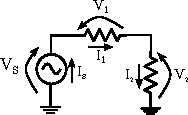
\includegraphics{weerstandsdeler}
				\caption{Elektronisch netwerk: een schakeling van componenten. Er is \textbf{over} elk component een spanningsval , en \textbf{door} elk component een stroom.}
				\label{subfig:netwerk}
			\end{subfigure}
			\caption{Componenten en een schakeling. }
			\label{fig:component_en_schakeling}
		\end{figure}

		 Elektrische ladingen gedragen zich verdacht veel zoals water\footnote{Er werd lang effectief gedacht dat elektriciteit een vloeistof was, de benamingen stroom en spanning stammen nog uit die tijd (\url{http://galileoandeinstein.physics.virginia.edu/more_stuff/E&M_Hist.html})}.
		Een elektrisch netwerk kan dus voorgesteld worden als een aaneenschakeling van waterpompen, buizen, kleppen... Elektrische spanning wordt voorgestled als waterdruk, en stroom als waterstroom. Omdat je als kind (hopelijk) meer met water hebt gespeeld dan met elektriciteit, gaat het vaak sneller om het waternetwerk te begrijpen.


		Heel de magie van de elektronica zit in de I tot V (stroom-spanning) functies waaraan de componenten voldoen. Die functies zijn gevonden met behulp van de fysica, en worden door ingenieurs gebruikt om netwerken te ontwerpen. We beginnen met de eenvoudigste (en \'e\'en van de belangrijkste) component: de weerstand.

		\subsection{De weerstand}
			\begin{figure}[htbp]
				\centering
				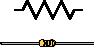
\includegraphics{weerstand}
				\caption{De weerstand: schematische voorstelling en re\"eel component.}
				\label{fig:weerstand}
			\end{figure}
			 Een weerstand is een geleider die voldoet aan de \textbf{wet van Ohm} die zegt dat de stroom en spanning evenredig zijn: 
			\begin{align}
				V &= R \cdot I
			\end{align} 
			$R$ heeft de eenheid Ohm\footnote{Georg Simon Ohm (1787 - 1854) was een Duits wiskundige en natuurkundige, ontdekker van de wet van Ohm in 1827.} ($\Omega$). De richting van de pijlen van stroom en spanning is belangrijk (figuur \ref{fig:weerstand}) !

			Het waterequivalent van een weerstand is een vernauwde buis (figuur~\ref{fig:waterweerstand}). De hoeveelheid water dat stroomt door de buis hangt af van het drukverschil tussen de uiteinden en de versmalling.

			\begin{figure}[htbp]
				\centering
				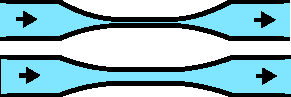
\includegraphics{waterweerstand}
				\caption{De waterweerstand. Hoe groter de weerstand, hoe nauwer de buis.}
				\label{fig:waterweerstand}
			\end{figure}
				\begin{DIY}
					Als ik een vaste spanning (bvb. 9V) heb en ik een grote stroom wil hebben door een weerstand, welke weerstand gebruik ik dan best?
					\begin{enumerate}[a)]
						\item een grote weerstand (hoge $R$)
						\item een kleine weerstand (kleine $R$)
					\end{enumerate}
				\end{DIY}

		\subsubsection{Serie en parallel}
			\label{sssec:serie_en_parallel}
			Twee weerstanden kunnen door \'e\'en  weerstand worden vervangen in twee gevallen (zie figuur \ref{fig:serie_en_parallel}):

			\begin{enumerate}
				\item twee weerstanden in \textbf{in serie} vormen de weerstand:
				\begin{align}
					R_{v} = R_1 + R_2.
				\end{align}
				Door weerstanden in serie te plaatsen, krijg je altijd een grotere weerstand.

				\item twee weerstanden in \textbf{parallel} vormen de weerstand:
				\begin{align}
					\frac{1}{R_{v}}= \frac{1}{R_{1}} + \frac{1}{R_{2}} 
				\end{align}
				Door weerstanden in parallel te plaatsen, krijg je altijd een kleinere weerstand.
			\end{enumerate}

			\begin{figure}[hbtp]
				\centering
				\begin{subfigure}[b]{0.3\linewidth}
					\centering
					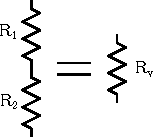
\includegraphics{serie}
					\caption{Weerstanden in serie.}
					\label{subfig:serie}
				\end{subfigure}
				~
				\begin{subfigure}[b]{0.3\linewidth}
					\centering
					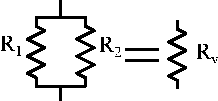
\includegraphics{parallel}
					\caption{Weerstanden in parallel.}
					\label{subfig:parallel}
				\end{subfigure}
				\caption{Serie en parallel.}
				\label{fig:serie_en_parallel}
			\end{figure}

			Niet alle weerstandswaarden bestaan in de handel, ze worden gemaakt in series met vaste waarden, zoals de E12 of E24 series (figuur \ref{fig:e12}). Het is dan de taak van een ingenieur om in te schatten welke waarde we het best gebruiken. 

			\begin{figure}[htbp]
				\centering
				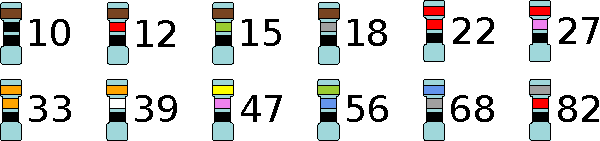
\includegraphics[scale=0.8]{e12}
				\caption{
				De vaak gebruikte E12 weerstanden-serie
				De kleurencode van de weerstand geeft de waarde aan. De weerstanden die bestaan zijn deze waarden, of tienvouden ervan. Bijvoorbeeld: de weerstanden 0.47 $\Omega$,  4.7 $\Omega$,47 $\Omega$, 470 $\Omega$, 4.7 k$\Omega$, etc\ldots (Fig. door \href{https://en.wikipedia.org/wiki/User:Pengo}{Peter Halasz})
				} 
				\label{fig:e12}
			\end{figure}

		\subsection{De spanningsbron}

			\begin{figure}[hbtp]
				\centering
				\begin{subfigure}[b]{0.25\linewidth}
					\centering
					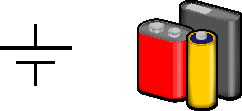
\includegraphics[width=\linewidth]{vc}
					\caption{Constante (DC) spanningsbron, bvb. batterijen.}
				\end{subfigure}
				~
				\begin{subfigure}[b]{0.25\linewidth}
					\centering
					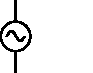
\includegraphics[width=\linewidth]{vt}
					\caption{Vari\"erende (AC) spanningsbron, bvb. de stropcontact die een een sinus van 230~V aanlegt.}
				\end{subfigure}
				~
				\begin{subfigure}[b]{0.25\linewidth}
					\centering
					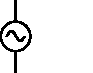
\includegraphics[width=\linewidth]{vt}
					\caption{Sleche bron.}
				\end{subfigure}

				\caption{Spanningsbronnen.}
				\label{fig:vbron}
			\end{figure}
			 Een perfecte spanningsbron is een simpel elektronisch component met twee pinnen die gehoorzaamt aan een eenvoudige wet: de spanningsbron legt de spanning over zijn pinnen op, onafhankelijk van de rest van het netwerk.
			 
			 In werkelijkheid kan een spanningsbron maar een beperkte stroom leveren en gedraagt zich dan als een perfecte spanningsbron met een kleine weerstand in serie. 
			 
			 Twee types bron bestaan: DC-bronnen die een vaste waarde aanleggen, of AC-bronnen die een signaal kunnen aanleggen zoals bvb. een sinus. Beide type bronnen hebben een verschillende schematische voorstelling die je kan vinden in figuur \ref{fig:vbron}.

			 Het waterequivalent is een pomp zijn die de druk tussen zijn uiteinden vastlegt of een watertoren die waterdruk druk genereert omwille van zijn hoogteverschil met de rest van het water (figuur \ref{fig:waterbron}).

		\begin{figure}[htbp]
				\centering
				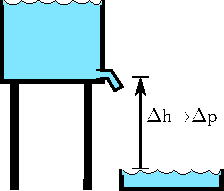
\includegraphics{waterbron}
				\caption{De waterdrukbron, die een drukverschil oplegt tussen de grond en zijn uiteinde.}
				\label{fig:waterbron}
			\end{figure}

			We gaan binnenkort wetten ontdekken van nog meer componenten, maar met onze voorlopige kennis kunnen we al volgend netwerk oplossen!

		
			\begin{DIY} 
			\begin{figure}[h!]
				\centering
				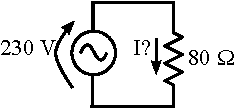
\includegraphics{vbweerstand.pdf}
				\caption{Voorbeeldnetwerkje.}
				\label{fig:vbweerstand}
			\end{figure}
			Een spanningsbron legt een wisselspanning (AC) op met een amplitude van $230~V$ over een weerstand van $80~\Omega$. (Dit is wat er gebeurt in een broodrooster, de weerstand is de gloeidraad die opwarmt en het brood bakt!) Wat is de amplitude van de  stroom $I$ door de weerstand? Wat is het elektrisch vermogen $P$ van de weerstand, die dan in warmte wordt omgevormd?
			\begin{align}
			    I&= \ldots & P&= \ldots 
			\end{align}
			\end{DIY}



		\subsection{De capaciteit}
		Een capaciteit of condensator (figuur \ref{fig:capaciteit}) is een component waar de stroom bepaald wordt door de maat van verandering van de spanning. De formele definitie van de stroom-spanning relatie is :
		\begin{align}
		    I = C \cdot \frac{dV}{dt}
		\end{align}
		met $C$ de capaciteitswaarde in Fahrad (F). 
		\begin{figure}[htbp!]
			\centering
			\begin{subfigure}[b]{0.45\linewidth}
				\centering
				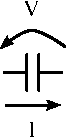
\includegraphics{cap}
				\caption{Symbool voor capaciteit}
			\end{subfigure}
			~
			\begin{subfigure}[b]{0.45\linewidth}
				\centering
				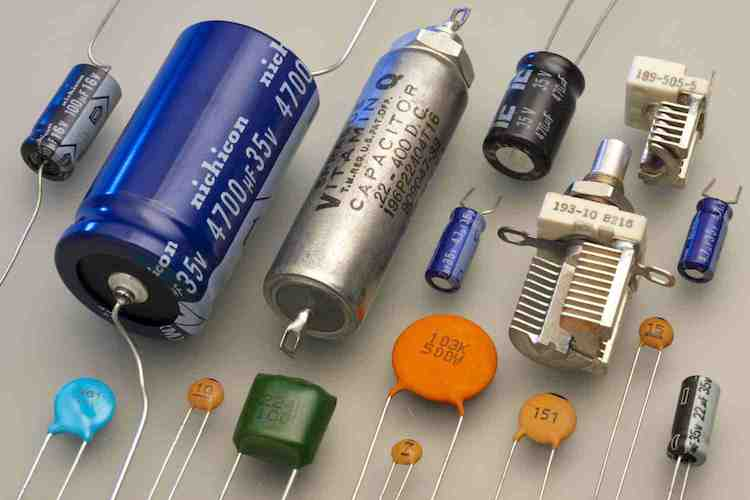
\includegraphics[scale=0.6]{caps}
				\caption{Capaciteiten in alle geuren en kleuren.}
			\end{subfigure}
		\caption{De capaciteit.}
		\label{fig:capaciteit}
		\end{figure}
		Een diepgaande studie van de capaciteit is tijdrovend en nutteloos voor onze toepassing, wij gaan capaciteiten enkel  gebruiken voor twee functies:
		\begin{enumerate}
			\item Ontkoppeling: Omdat een capaciteit alleen reageert op verandering van spanning, laat het geen DC stroom door. We gaan dit gebruiken om AC signalen door te laten, maar DC signalen tegen te houden.
			\item Hulpbatterij: capaciteiten kunnen zich gedragen zoals mini-batterijen die veel stroom kunnen leveren op een korte tijd, dit kan helpen wanneer de schakeling meer stroom vraagt dan de batterij kan leveren.\footnote{ Een voorbeeld daarvan is de defibrillator, waar een hoogspanningscapaciteit wordt opgeladen, en in \'e\'en schok wordt ontladen op het hart van een pati\"ent.}
		\end{enumerate}
		Pas op: zogenaamde elektrolytische capaciteiten hebben een richting, die mag je niet omgekeerd plaatsen. De richting wordt aangeduid met een + op een van de pinnen.

		Het waterequivalent van de capaciteit is een rubberen membraan in een buis, de capaciteitswaarde stelt dan de dikte van de membraan voor. Je kan door een membraan niet constant water laten stromen, anders gaat het stuk. Maar als er het water heen en weer gaat, gaat de membraan bewegen en de golf doorgeven. 
		\begin{figure}[htbp]
				\centering
				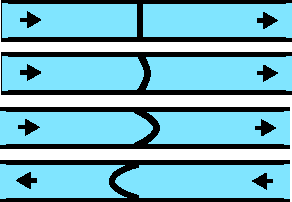
\includegraphics{watercap}
				\caption{De watercapaciteit, die kan voorgesteld worden als een rubberen membraan. De stroomrichting aangegeven met pijlen.}
				\label{fig:watercap}
			\end{figure}

		Elektronica is meer dan een componenten op hun eigen, ze moeten geschakeld worden in netwerken! Laten we maar een zien hoe netwerken zich gedragen.

		\subsection{Netwerken}

			Een netwerk is een aaneenschakeling van componenten, die schematisch wordt voorgesteld zoals in figuur \ref{subfig:netwerk}. Een netwerk is gemaakt uit \textbf{takken}  met componenten op die verbonden zijn via \textbf{knooppunten}. 

			 Er zijn maar twee regels die gelden voor elektrische/elektronische netwerken: de wetten van Kirchhoff\footnote{Gustav Robert Kirchhoff (1824 - 1887) was een Duits natuurkundige. Kirchhoff formuleerde zijn spanningswet en zijn stroomwet in 1845, toen hij nog een student was. Slimme kerel!}. Samen met de fysische wetten van de componenten kan je dan alle netwerken van de wereld oplossen. Een netwerk oplossen wilt zeggen dat je alle stromen en spanningen bepaalt in dat netwerk.

			\paragraph*{De stroomwet van Kirchhoff:} in elk knooppunt in een elektrische kring is de som van de stromen die in dat punt samenkomen gelijk aan de som van de stromen die vanuit dat punt vertrekken. Dit is voor elk knooppunt geldig, onafhankelijk van de componenten die op de takken zijn. 
			\paragraph*{De spanningswet van Kirchhoff:} de som van de elektrische potentiaalverschillen (rekening houdend met de richting) in elke gesloten lus in een kring is gelijk aan nul. 

			\begin{figure}[htbp!]
				\centering
				\begin{subfigure}[b]{0.45\linewidth}
					\centering
					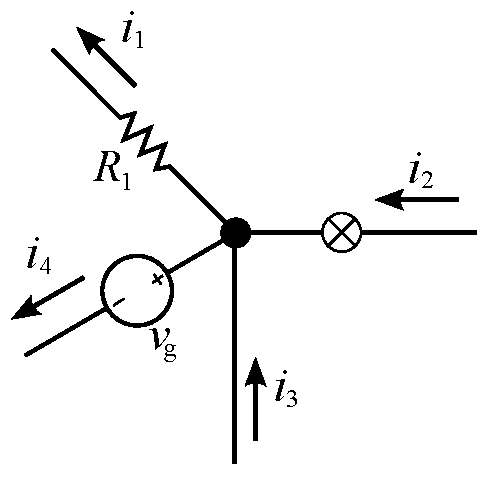
\includegraphics[scale=0.5]{kcl.pdf}
					\caption{In dit knooppunt is de stroomwet van Kirchhoff : $i_1 + i_4 = i_2+i_3$}
					\label{subfig:kcl}
				\end{subfigure}
				~
				\begin{subfigure}[b]{0.45\linewidth}
					\centering
					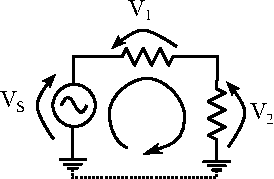
\includegraphics{kvl.pdf}
					\caption{In deze lus is is de spanningswet van Kirchhoff : $ + V_S - V_1 - V_2 = 0$}
					\label{subfig:kvl}
				\end{subfigure}
			\caption{De wetten van Kirchhoff}
			\label{fig:kirchoff}
			\end{figure}

			% \paragraph*{Voorbeeld:} De stroomwet (figuur \ref{subfig:kcl}) wordt toegepast als volgt: kies een knooppunt in een netwerk. Beschouw alle takken die dat knooppunt raken, en de bijhorende stromen. Als je alle stromen optelt die \textbf{naar} het knooppunt wijzen, dan is dat gelijk aan alle stromen die \textbf{weg} van het knooppunt wijzen.

			% Voor dat we spanningswet toepassen, hebben we de betekenis van het symbool 
\includegraphics[height=1em]{gnd.pdf} nodig. Dit symbool wordt de \textbf{grond} genoemd. Het is geen component, maar een manier aan te duiden dat alle punten met dat symbool verbonden zijn. Je mag dus een connectie tekenen tussen alle pinnen die aan de grond verbonden zijn. Vergeet niet dat een spanning altijd gedefini\"eerd is tussen twee punten, vaak wordt de grond gebruikt als een van die twee punten, en we zeggen dat de grond op 0 V is.

			% \paragraph*{Voorbeeld:} De spanningswet (figuur \ref{subfig:kvl}) pas je zo toe: vind een gesloten lus in het netwerk (vergeet niet dat alle pinnen aan grond met elkaar verbonden zijn). Teken een lus met een zekere richting in het netwerk. Schrijf de som van de spanningen rekening houdend met de volgende regels:

			% \begin{enumerate}
			%  	\item Als de spanning in dezelfde richting gaat als de lus, dan krijgt die een positief teken.
			%  	\item Als de spanning tegen de lus ingaat, dan krijgt die een negatief teken.
			%  \end{enumerate}

			% \paragraph*{Fun fact:} Je kan de vergelijkingen voor serie en parallel weerstanden (sectie \ref{sssec:serie_en_parallel}) afleiden met behulp van de wetten van Kirchhoff en de wet van Ohm.

			\begin{DIY} Pas de stroomwet van Kirchhoff toe in figuur \ref{subfig:kcl_oef}, en vind de missende stromen. Doe hetzelfde voor de spanningen in figuur \ref{subfig:kvl_oef}.
			\begin{align*}
			    I_S &= \ldots & V_1 = \ldots\\
			    I_R &= \ldots & V_2 = \ldots
			\end{align*}
			\end{DIY}

			\begin{figure}[htbp]
				\centering
				\begin{subfigure}[b]{0.45\linewidth}
					\centering
					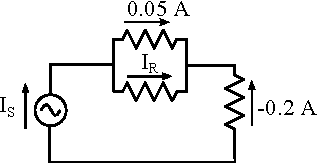
\includegraphics{kcl_oef.pdf}
					\caption{Vind $I_R$ en $I_s$.}
					\label{subfig:kcl_oef}
				\end{subfigure}
				~
				\begin{subfigure}[b]{0.45\linewidth}
					\centering
					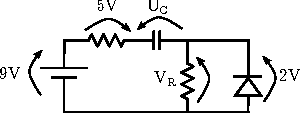
\includegraphics[width=\linewidth]{kvl_oef.pdf}
					\caption{Vind $V_R$ en $U_C$. }
					\label{subfig:kvl_oef}
				\end{subfigure}
			\caption{De wetten van Kirchhoff}
			\label{fig:kirchoff_oef}
			\end{figure}

			Dit be\"eindigt de kennismaking met de elektronica. Je hebt nu alle basis die nodig is om aan de bouw van een versterker te beginnen! Daar gaan we alleen nieuwe componenten leren kennen zoals de diode en de transistor, maar voor de rest komt er niets nieuws onder de zon!

	\section{Bouwstenen van de e-VUBOX}
	\label{sec:bouwstenen}
		In dit deel gaan we stap voor stap de onderdelen van onze versterker ontwerpen die je kan vinden in  figuur \ref{fig:pcb}. Elke keer dat we een componentswaarde hebben berekend, kan je het alvast overschrijven op het elektrisch schema op de laatste pagina (figuur~\ref{fig:volledig_schema}). 

		\begin{figure}[htbp]
				\centering
				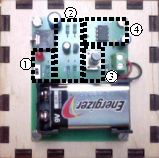
\includegraphics[scale=3]{pcb}
				\caption{Het circuit met de onderdelen die we gaan ontwerpen. 1) Statusledje 2) Versterker 3) Volumeknopje 4) Ge\"integreerde schakeling}
				\label{fig:pcb}
			\end{figure}

		\subsection{Introductie: het versterken van audio}

			Ook als je een student in elektronisch ingenieur bent, is een basiskennis in de rest van de wetenschappen toch handig. Want hoe versterk je geluid?

			Je weet dat geluid een drukgolf is door lucht. We kunnen een drukgolf uitdrukken als een sinus, met bijvoorbeeld een frequentie van $440$ Hz (dit is de muzieknoot la):
			\begin{align}
				y(t) = A \cdot \sin (2\pi \cdot 440~\text{Hz} \cdot t)
			\end{align}
			met $y(t)$ de luchtdruk in Pascal, $A$ de amplitude van de drukgolf in Pascal en $t$ de tijd in seconden.
			Om het te versterken moeten we eerst de drukgolf omzetten naar een elektronengolf, die we gaan versterken, en dan terug naar een drukgolf zodat we het kunnen horen. Daarvoor gebruiken we twee componenten die je zeker kent: de microfoon en de luidspreker.
			De microfoon gaat die drukgolf omvormen naar een spanningsgolf, met dezelfde frequentie (zie figuur \ref{fig:micro}). Om de muziek te kunnen horen gebruiken we een luidspreker, die exact het omgekeerde doet van een microfoon. 

			\begin{figure}[htbp]
				\centering
				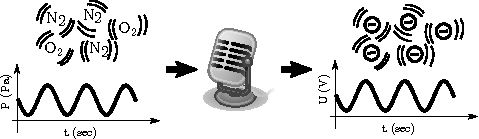
\includegraphics[scale=1.2]{micro}
				\caption{Een microfoon vormt de luchtdrukgolf (eenheid: Pascal) om in een spanningsgolf (eenheid: Volt), een luidspreker doet het omgekeerde.}
				\label{fig:micro}
			\end{figure}


			Om luid muziek te kunnen afspelen, moet er veel energie gepompt worden in de luidspreker. Anders gezegd moet het vermogen gebruikt door de luidspreker groot zijn. Dat is het  doel van een versterker: het vermogen van de muziek groot maken! Nu dat we weten waarom ons netwerk nuttig is, kunnen we aan de bouw van onze versterker beginnen! Het ontwerpen van een versterker is, zoals je het zult zien, meestal het kiezen van enkele weerstandswaarden.

		\subsection{De volumeknop: de spanningsdeler}

			De weerstandsdeler is een basisonderdeel in elektrische schakelingen. Het is een onderdeel dat aan de uitgang een spanning levert dat een fractie is van de ingangspanning.

			 Stel dat een bron een muzieksignaal (AC) $V_s$ genereert, en dat we in serie met die spanningsbron twee weerstanden schakelen (figuur \ref{fig:volume}), dan hebben we een  \textbf{spanningsdeler} gebouwd. 

			 We gaan aantonen de spanning $V_1$ een verkleinde versie is van het muzieksignaal $V_s$.

			\begin{figure}[htbp]
				\centering
				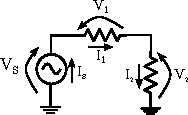
\includegraphics{weerstandsdeler}
				\caption{Volumeregeling: de spanningsdeler}
				\label{fig:volume}
			\end{figure}

			We gaan op zoek naar de uitgangsspanning $V_1$. De stroom in het circuit is overal dezelfde (serieweerstanden en wet van Ohm):
			\begin{align}
			    I &= \frac{V_S}{R_1 + R_2}
			\end{align}
			De spanning $V_1$ vinden we met de wet van Ohm:
			\begin{align}
			    V_1 = \frac{R_1}{R_1+R_2} \cdot V_S
			\end{align}

			Je kan zien dat de spanning $V_1$, die we de uitgangsspanning noemen, altijd kleiner is dan (of gelijk aan) de ingangsspanning $V_s$. Daarom noemen we dit een spanningsdeler.

			\begin{DIY}
				Je hebt een voltage van $9$ V als ingangsspanning $V_S$, en je wilt een voltage van $1.5$ V als uitgangsspanning $V_2$. $R_1$ is al gekozen en heeft een weerstand van $1$ k$\Omega$ ($1000 \Omega$). Welke waarde moet je kiezen voor $R_2$?
				
				\begin{align*}
				    R_2 = \ldots\ldots
				\end{align*}

				Let op! Bestaat die weerstandswaarde wel? Kies een bestaande waarde uit de E12-reeks in figuur \ref{fig:e12} op pagina \pageref{fig:e12}.
			\end{DIY}

			Weerstandsdelers worden vaak gebruikt in netwerken om een specifieke spanning te verkrijgen vanuit een grotere spanning.
			Wanneer een spanningsdeler met een regelbare weerstand word gemaakt (zie figuur \ref{subfig:regelbareR}), heb je een volumeknop! De combinatie $R_1R_2$ kan gemaakt worden met een enkele regelbare weerstand, of \emph{potentiometer} (figuur \ref{subfig:pot}).

			\begin{DIY} Welke weerstand $R_{pot}$ moet de potentiometer hebben, wetend dat de ingangsspanning $V$ maximaal $200$ mV ( = $200 \cdot 10^{-3}$ V) is en we het vermogen $P$ door de potentiometer willen beperken tot 4 $\mu$W ( = $4 \cdot 10^{-6}$ W)? 
			\begin{align*}
			    R_{pot} = \ldots\ldots
			\end{align*}
			\end{DIY}			

			Schrijf de waarde die je hebt gevonden voor $R_{pot}$ over in de schakeling op de laatste pagina.
			\begin{figure}
				\centering
				\begin{subfigure}[b]{0.45\linewidth}
					\centering
					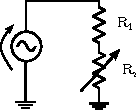
\includegraphics{regelbareR}
					\caption{Spanningsdeler met een regelbare weerstand (weerstand met een pijltje).}
					\label{subfig:regelbareR}
				\end{subfigure}
				~
				\begin{subfigure}[b]{0.45\linewidth}
					\centering
					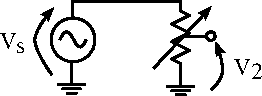
\includegraphics{potentiometer.pdf}
					\caption{Spanningsdeler met een potentiometer.}
					\label{subfig:pot}
				\end{subfigure}
			\caption{Types spanningsdelers.}
			\label{fig:vdeler} 
			\end{figure}

		\subsection{Het statusledje: de diode}

			Een handig onderdeel op veel elektronische toestellen is het ledje dat brandt om aan te geven dat het toestal aan is, en dat de batterij nog werkt. LED staat voor Light Emitting Diode, lichtdiode\footnote{Niet alle diodes zijn lichtgevend, diodes zijn ook nuttig voor andere toepassingen.}. Een diode (figuur \ref{fig:diode}) is een component die alleen stroom doorlaat in de positieve stroomrichting (van + naar -). Het waterequivalent is eenvoudigweg een \'e\'enrichtingsklep.
			\begin{figure}[htbp]
			\centering
				\begin{subfigure}[b]{0.45\linewidth}
					\centering
					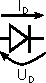
\includegraphics{diode}
					\caption{Een diode met voorwaartse spanning $U_D$ en stroom $I_D$. De diode laat alleen stroom toe in de  positieve stroomrichting , van de anode (+) naar de kathode (-).}
					\label{fig:diode}
				\end{subfigure}
				~
				\begin{subfigure}[b]{0.45\linewidth}
					\centering
				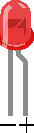
\includegraphics[width=0.1\textwidth]{led}
				\caption{Rood ledje.}
				\label{fig:led}
				\end{subfigure}
				\caption{De Diode}
			\end{figure}

			In figuur \ref{fig:diode_grafiek} zie je de grafiek van de stroom in functie van de spanning van de diode die we gaan gebruiken in onze versterker. In tegenstelling met de weerstand is de fysische wet van de diode niet-lineair (= het is geen rechte): het is een exponenti\"ele functie. Als je het voltage verdubbelt over de diode, gaat de stroom niet verdubbelen, maar exponenti\"eel groter worden.
				\begin{figure}[htbp]
					\centering
					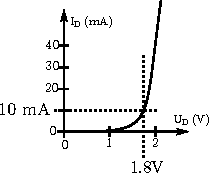
\includegraphics{diode_grafiek}
					\caption{Grafiek van de stroom in functie van de spanning van een diode.}
					\label{fig:diode_grafiek}
				\end{figure}
				
			Omdat rekenen met een exponenti\"ele functie tijdrovend is, gaat een ingenieur meestal eerst proberen om zich te redden met de grafiek. We gaan het circuit in figuur \ref{fig:diode_netwerk} oplossen zonder de die moeilijke functie te gebruiken.

			\begin{figure}[htbp]
				\centering
				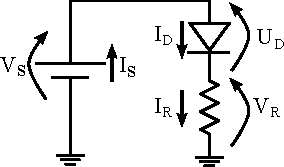
\includegraphics{diode_netwerk}
				\caption{Diode netwerk.}
				\label{fig:diode_netwerk}
			\end{figure}

			We kiezen de stroom $I_D$ dat door de LED vloet, dat bepaalt de lichtintensiteit. De datasheet\footnote{Een datasheet is een document dat de eigenschappen van elektronische componenten beschrijft.} zegt dat $10$ mA een typische stroomwaarde is voor onze LED. Op het grafiek \ref{fig:diode_grafiek} zien we dat de spanning over de diode dan $1.8 $V moet zijn (Deze waarde hangt af van de kleur van de LED). 

			Dankzij een weerstand kunnen we een netwerk maken die zeker maakt dat de stroom en spanning die we gekozen hebben voor onze led worden opgelegd (figuur \ref{fig:diode_netwerk}).
			
			\begin{DIY}
				De spanningsbron die we gaan gebruiken voor onze versterker is een 9V batterij, dus $V_s = 9$ V. We zijn op zoek naar de weerstand die nodig is zodat de $U_D = 1.8$ V en $I_D =10$ mA. Gebruik de wetten van Kirchhoff:
				\begin{align}
					+V_s &- U_D - V_R = 0  \\
					I_s &= I_D = I_R
				\end{align}
				 Kan je de waarde vinden van de weerstand die nodig is? \textbf{Tip:} bepaal $I_R$ en $V_R$ uit de wetten van Kirchhoff.
				\begin{align*}
				    R_{led} = \ldots\ldots
				\end{align*}
			\end{DIY}

			Kies zeker een E12-weerstand en schrijf de waarde over in de schakeling op pagina \pageref{fig:volledig_schema}.
			We gaan een mechanische schakelaar plaatsen tussen de bron en de diode zodat het licht alleen brandt wanneer het toestal aan is.

		\subsection{De versterker: de transistor}

			De transistor is een actieve elektronische component uitgevonden in $1947$, en is het basisingredi\"ent van alle elektronische netwerken, van simpele versterkers tot een volledige PC. In tegenstelling tot \emph{passieve} componenten zoals de diode en de weerstand hebben \emph{actieve} componenten nood aan een voeding, een externe energiebron die nodig is om ze te laten werken. Ze kunnen dankzij die extra energiebron (bvb. een batterij) energie inpompen in een netwerk, en zijn dus handig voor versterking.

			\begin{figure}[htbp]
				\centering
				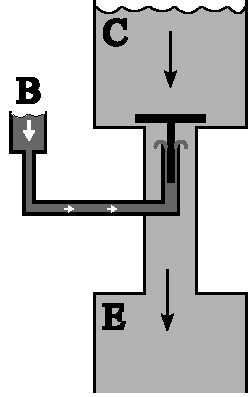
\includegraphics[width=0.3\textwidth]{watertransistor}
				\caption{Hydraulische analogie van de transistor.}
				\label{fig:watertransistor}
			\end{figure}

			We gaan de werking van de transistor uitleggen met zijn waterequivalent (figuur \ref{fig:watertransistor}). De watertransistor werkt als volgt: als er geen stroom vloeit in de basis (B), dan sluit het ventiel het contact tussen collector (C) en emitter (E), er loopt geen stroom door de transistor. Een kleine stroom in de basis drukt het ventiel naar boven, en er kan een grote stroom lopen van de collector naar de emitter. Een kleine stroom veroorzaakt dus een grote stroom, en dat is het principe van de versterkerwerking van een transistor! Er is wel een externe energiebron nodig om die grote stroom te kunnen blijven leveren, bij de watertransistor zou dat een watertoren kunnen zijn dat aangesloten is aan de collector.

			
			\subsubsection{De bipolaire npn transistor}
				 Transistoren bestaan in verschillende types, wij gaan ons beperken tot de \emph{bipolaire NPN} transistor. Zoals je kan zien in figuur \ref{subfig:transistor_bce} is het een component met 3 pinnen, die elk een naam dragen: de basis, de collector en de emitter.
				\begin{figure}[htbp]
				\centering
					\begin{subfigure}[b]{0.45\linewidth}
						\centering
					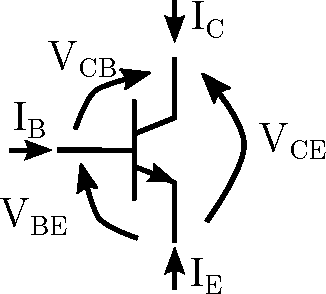
\includegraphics{transistor_VI}
					\caption{Schematische voorstelling van de bipolaire transistor met stromen en spanningen. Alle stromen worden conventioneel \textbf{naar} de transistor toe getekend.}
					\label{subfig:transistor_vi}
					\end{subfigure}
					~
					\begin{subfigure}[b]{0.45\linewidth}
						\centering
						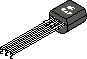
\includegraphics[scale=2]{transistor}
						\caption{De BC547 bipolaire transistor met Basis, Collector en Emitter aangeduid.}
						\label{subfig:transistor_bce}
					\end{subfigure}
					
					\caption{De bipolaire npn transistor.}
					\label{fig:transistor}
				\end{figure}

				De fysische wetten die de relatie geeft tussen de stromen en de spanningen noemen de Ebers-Moll vergelijkingen. Zoals met de diode worden die niet vaak gebruikt tijdens het ontwerp, omdat ze te complex zijn. We kunnen dan  de grafieken gebruiken, maar voor de bipolaire transistor is er nog een derde weg: enkele regeltjes volstaan om te kunnen ontwerpen. 

				De regels waaraan een bipolaire transistor zich moet houden zijn:
				\begin{enumerate}
					\item De spanning op collector moet positiever zijn dan die op de basis: 
					\item De spanningsval tussen basis en emitter is ongeveer $0.7$ V.
					\item $I_C, I_B$ en $V_{CE} $ moeten binnen bepaalde maximale waarden liggen, of de transistor gaat stuk (een transistor kan letterlijk in brand schieten, let op!). Die maximale waarden verschillen van model tot model.
					\item Als aan de drie vorige regels is voldaan, dan is de collectorsstroom een versterkte versie van de basisstroom.
				\end{enumerate}
				Wiskundig kunnen we dit schrijven als:
					\begin{align}
					    V_{CB} &> 0~V. \\
						V_{BE} &\approx 0.7~V \\
					    I_C &= \beta I_B
					    \label{eq:hfe}
					\end{align}
					$\beta$ (ook als $h_{FE}$ genoteerd) wordt de stroomversterkingsfactor genoemd, en is typisch ten minste $50$, maar kan veel groter zijn. Dit is waarom de transistor nuttig is: een minuscuul kleine basisstroom controleert een veel grotere collectorstroom.


				De wetten van Kirchhoff gelden ook voor de transistor\footnote{We hebben hier eigenlijk de ``algemene'' wetten van Kirchoff gebruikt, waarvan de wetten van Kirchhoff die we hebben gezien zijn afgeleid. We kunnen inderdaad hier niet echt een knooppunt en een lus defin\"eren in het ``midden'' van de transistor.}:
				\begin{align}
				    I_C		&+ I_B = -I_E \\
				    V_{BE}  &+ V_{CB} - V_{CE} = 0
				\end{align}

				Spijtig gnenoeg is de stroomversterkingsfactor $\beta$ van een transistor is niet echt een te vertrouwen waarde: het kan afhangen van temperatuur, waar en wanneer het gemaakt werd, enz\ldots). We hebben dus liever dat het niet voorkomt in onze vergelijkingen. Met de stroomwet van Kirchoff en vergelijking (\ref{eq:hfe}) kunnen we volgende relatie vinden:
				\begin{align}
				    I_C = -\frac{\beta}{\beta+1}I_E
				\end{align}

				\begin{DIY}
					Elimineer $\beta$ van de vorige vergelijking door de volgende limiet op te lossen.
					\begin{align*}
					    \lim_{\beta \rightarrow \infty} I_C = \lim_{\beta \rightarrow \infty} -\frac{\beta}{\beta+1}I_E = \ldots
					\end{align*}
				\end{DIY}

				Een negatieve stroom is perfect mogelijk, dat wilt gewoon zeggen dat de stroom loopt tegen de pijlrichting in van figuur \ref{subfig:transistor_vi}. Bijna alle stroom die in de collector vloeit gaat dus via de emitter terug naar buiten. We gebruiken die vergelijking liever dan vergelijking \ref{eq:hfe} zodat we $\beta$ niet gebruiken.

			\subsubsection{Het versterkingsnetwerk}
				In figuur \ref{fig:ges} vind je onze audioversterker, waar je de bipolaire transistor in herkent. Je ziet dat we een actief netwerk hebben, er is een externe energiebron: de batterij $V_{CC}$. Het muzieksignaal dat we gaan versterken is in de spanningsbron $V_S$.

				\begin{figure}[htbp]
					\centering
					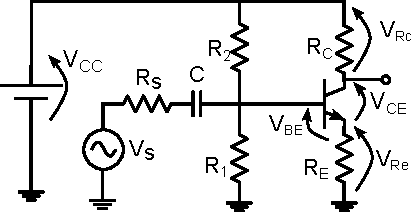
\includegraphics{ges}
					\caption{Versterkerschakeling met de transistor.}
					\label{fig:ges}
				\end{figure}

				$R_s$ is de serieweerstand van de spanningsbron, en $C$ is een ontkoppelcapaciteit (laat geen DC door).

				Om de versterker te ontwerpen moeten we de weerstanden $R_1,R_2,R_E$ en $R_C$ kiezen. Een eerste vergelijking die belangrijk gaan we nu afleiden: de spanningsversterking van dit netwerk. ($V_B$ is de spanning van de basis ten opzichte van de grond, analoog voor $V_E$ en $V_C$). Probeer zeker de redenering te volgen met het schema! 

				 \begin{align*}
				     \intertext{De ingangspanning $V_B$ bepaalt de spanning $V_E$ dankzij de transistor:}
				     V_{BE} &= V_B - V_E = 0.7~V \\
				     V_E &= V_B - 0.7~V \\
				     \intertext{De spanning $V_E$ veroorzaakt een stroom door de weerstand $R_E$ (met minteken omdat $I_E$ en $V_E$ dezelfde pijlrichting hebben)}
				     I_E &= -\frac{V_E}{R_E} = -\frac{V_B - 0.7~V}{R_E}
				     \intertext{Weeral omwille van de transistor gaat dezelfde stroom lopen door de weerstand $R_C$:}
				     I_C &= - I_E = \frac{V_B - 0.7~V}{R_E}
				     \intertext{De spanning over de weerstand $R_C$ is dan:}
				     V_{R_C} &= R_C \cdot I_C = \frac{R_C}{R_E} \cdot (V_B - 0.7~V)
				     \intertext{Je ziet al dat de verhouding van $R_C$ en $R_E$ de spanning bepaalt. We drukken als laatste stap de spanning $V_C$ uit:}
				     V_C &= V_{CC} - V_{R_C} = V_{CC} - \frac{R_C}{R_E} \cdot (V_B - 0.7~V)
				     \label{eq:versterking}
				 \end{align*}

				\begin{DIY}
					Door de ontkoppelcapaciteit $C$ en de weerstandsdeler $R_1R_2$ is
					\begin{align*}
					    V_B = \frac{R_1}{R_1+R_2}V_{CC} +V_S
					\end{align*}
					 $V_{CC}$ is een DC spanning, de muziek $V_S$ is een AC spanning. Vul dit in vergelijking \ref{eq:versterking}, en  splits de spanning $V_C$ op in een AC en DC gedeelte:
					\begin{align*}
					    (AC)~v_C = \ldots \\ (DC)~V_C = \ldots & 
					\end{align*}
				\end{DIY}

				Deze schakeling versterkt dus de AC spanning met een factor $- \frac{R_C}{R_E}$, de muziekgolf wordt dus omgedraaid en de amplitude versterkt! De andere DC waarden wilt alleen zeggen dat het gemiddelde van de golf zich verplaatst, zoals je kan zien in figuur \ref{fig:golven}.

				\begin{figure}[htbp]
					\centering
					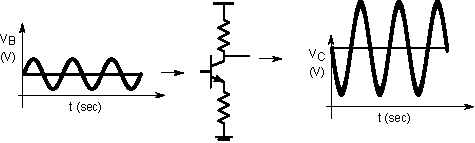
\includegraphics[width=\linewidth]{golven}
					\caption{De ingangsgolf wordt door ons netwerk omgedraaid, versterkt, en het gemiddelde verschuift.}
					\label{fig:golven}
				\end{figure}

				Tjongejonge, dat was heel een geworstel om tot die conclusie te komen... Gelukkig zijn we klaar met dingen af te leiden, we hebben alle informatie vergaard die nodig is om dit onderdeel te ontwerpen. 

				De keuze van $R_1$,$R_2$,$R_E$ en $R_C$ doen we met volgende ontwerpmethode. Eens je de methode kent, kan je andere keuzes proberen maken en zien als het werkt: dit is wat ontwerpen is. Niet alle designers gaan het graag zeggen, maar een groot deel van ontwerp is vallen en opstaan: uitproberen tot dat het werkt, en daar is niets mis mee!

				Zoals vaak bestaat de methode uit het kiezen van DC-waarden van enkele grootheden:
				\begin{enumerate}
					\item Kies de DC-waarde van de  stroom $I_C$. 

					De maximumwaarde die de BC 547 transistor aankan is $100~mA$, dus het moet kleiner. Te grote stromen gaan ook de batterij sneller leegzuigen, te kleine stromen kunnen de werking van het netwerk stopzetten. Er zijn nog  andere voor- en nadelen die je kan uitzoeken voor te grote of te kleine stromen. We kiezen bijvoorbeeld:
					\begin{align}
					    I_C = 10~mA
					\end{align}

					\item Kies een DC-voltage $V_C$.

					 De spanning $V_C$ moet groter zijn dan $0.7~V$ (dat kan je afleiden uit de spanningswet van Kirchhoff en  $V_{CB} > 0$, en $V_{BE} = 0.7$). De transistor kan hier de spanning aan zijn pinnen niet hoger krijgen dan zijn voeding. Het maximum is dus $V_{CC} = 9~V$. Pas op, een batterij gaat slijten, na een tijdje kan de geleverde spanning zo laag als $7~V$ gaan. De voorbeeldkeuze die wie hier maken is:
					\begin{align}
					    V_C =  3.5~V
					\end{align}
					 Dat is ongeveer in het midden tussen $7~V$ en $0.7~V$. Je kan snappen waarom het midden een mogelijke keuze is door een tekening te maken zoals in figuur \ref{fig:golven}. Dit is niet de enige mogelijkheid!

					\item Kies een versterkingsfactor $- \frac{R_C}{R_E}$. 

					Als je de amplitude van de inkomende golf $V_S$ kent, dan kan de versterkingsfactor zo kiezen dat je uitgaande spanningsgolf zeker niet boven $V_{CC}$ komt, of onder $0$ V (=de grond). Spijtig genoeg is er geen standaardwaarde voor de amplitude van een muzieksignaal, maar het is meestal klein en ongeveer  $200~mV$. We kunnen bijvoorbeeld zeggen dat we de amplitude naar $1V$ willen krijgen, we hebben dus een versterkingsfactor nodig van $-5$.
					\begin{align}
					    -\frac{R_C}{R_E} = -5
					\end{align}
				\end{enumerate}

				Vergeet niet dat dit niet vaste keuzes zijn, er zijn veel andere mogelijkheden, probeer vast en zeker te spelen met andere waardes!

				\begin{DIY} Je kent nu alles wat nodig is om de weerstanden $R_{E}$ en $ R_{C}$ te bepalen. \textbf{Tip:} Uit $I_C$ en $V_C$ kan je de waarde $R_C$ vinden.
				\begin{align}
				    R_C &= \ldots \\
				    R_E &= \ldots
				\end{align}
				\end{DIY}				

				De DC-waarde van $V_B$ ligt nu al vast (omdat $V_{BE} = 0.7V$), en noemen we het biaspunt. De weerstandsdeler dient om die DC-waarde op te leggen. Alhoewel het geen zuivere weerstandsdeler is (normaal gezien is niets aangesloten aan een weerstandsdeler), kunnen we toch de formule van de weerstandsdeler gebruiken hier.

				\begin{DIY} Bereken het biasvoltage $V_B$ uit $V_E$. Kies dan de weerstand $R_2$ zodat de uitgangspanning $V_B$ de gewenste waarde heeft. Het staat al vast dat $R_1 = 1k\Omega$. \textbf{Tip:} Vergeet niet de ingansspanning $V_{CC}$ is $9V$.
				\begin{align}
					V_B &= \ldots \\
				    R_1 &= 1k\Omega \\
				    R_2 &= \ldots
				\end{align}
				\end{DIY}

				Alle weerstanden zijn nu bepaald! Schrijf ze over in het elektronisch schema op pagina \ref{fig:volledig_schema}, vergeet niet E12 weerstanden te kiezen.

				Je kan nu zien dat we vermogen hebben versterkt van het ingangssignaal:
				\begin{enumerate}
				 	\item de amplitude van de stroom $I_B$ is enkele $\mu$A $\rightarrow$ de amplitude van $I_C$ is enkele mA
				 	\item de amplitude van de spanning $V_B$ is enkele mV $\rightarrow$ de amplitude van $V_E$ in de grootteorde van 1 Volt
				 \end{enumerate} 

				 De stroom en de spanning zijn  versterkt, dus het vermogen is gestegen! We zijn vertrokken van enkele $\mu$W en we hebben nu uiteindelijk enkele $m$W. 


%				\begin{center}
%					\noindent \fbox{ 
%						\parbox{0.8\textwidth}{
%							Samenvatting van de gekozen weerstanden:
%							\begin{align*}
%							    R_1 &= \ldots \\
%							    R_2 &= \ldots \\
%							    R_E &= \ldots \\
%							    R_C &= \ldots
%							\end{align*}
%						}
%					 }
%				\end{center}

		\subsection{De magische zwarte doos: de ge\"integreerde schakeling}
			Dankzij de transistor-schakeling hebben we meer vermogen, maar een luidspreker heeft enkele honderden milliwatts nodig om luid genoeg te klinken, dat is meer dan enkele milliwatts we nu hebben! We gaan dus het signaal nog eens versterken.

			Deze keer gaat onze aanpak verschillend zijn: we gaan de versterker niet zelf maken, maar gaan een IC (Integrated Circuit of ge\"integreerde schakeling) gebruiken die daarvoor gemaakt is, zodat we niet het warm water opnieuw uitvinden. Een IC is een volledig elektronisch netwerkje gemaakt op een plaatje silicium, die dan is verpakt in een behuizing uit kunststof met pinnetjes om het te verbinden met andere circuits, zoals je kan zien in figuur \ref{fig:IC}.

			\begin{figure}[htbp]
			\centering
				\begin{subfigure}[b]{0.45\linewidth}
					\centering
					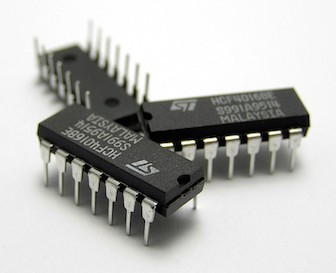
\includegraphics[width=0.7\textwidth]{IC}
					\caption{Voorbeelden van IC's, in een DIP (Dual-in-line Packaging) behuizing.}
					\label{subfig:IC_foto}
				\end{subfigure}
				~
				\begin{subfigure}[b]{0.45\linewidth}
					\centering
				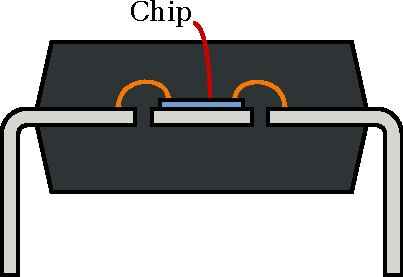
\includegraphics[width=0.5\textwidth]{IC_doorsnede}
				\caption{Doorsnede van een IC, het circuit (of chip) in de behuizing wordt verbonden met de buitenwereld via de pinnetjes. }
				\label{subfig:IC_doorsnede}
				\end{subfigure}
				\caption{Ge\"integreerde schakelingen.}
				\label{fig:IC}
			\end{figure}

			We gaan hier een IC gebruiken die gemaakt is om audio te versterken, de LM-386. IC's worden vaak benoemd met een combinatie van letters en getallen. Alle IC's hebben een handleiding die uitleg geeft over hun werking, die we een datasheet noemen. In de datasheet van de LM-386 staat hoe je het moet gebruiken om een versterker te maken met spanningsversterkingsfactor $20$.

			\begin{figure}[htbp]
				\centering
				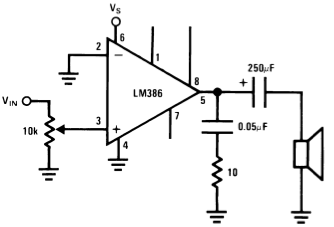
\includegraphics[width=0.6\textwidth]{IC_versterker}
				\caption{Schakeling uit de datasheet van de LM-386 voor een spanningsversterking van 20. De getallen duiden de pinnen aan van het IC, de driehoek is het symbool voor het IC. }
				\label{fig:IC_versterker}
			\end{figure}

			Een IC is niets magisch: het netwerk binnen de behuizing heeft vaak als basisingredi\"ent transistoren, en werkt in principe zoals de netwerken die we net hebben besproken, alleen op een veel kleinere schaal. Het ontwerpen van een IC is ook het werk van een ingenieur in de elektronica!

			Het praktische aan een IC is dat we nu al klaar zijn met de tweede versterkersstap: we moeten gewoonweg de schakeling in figuur \ref{fig:IC_versterker} bouwen. We vervangen de capaciteiten van $0.05 \mu$F en $250\mu$F door capaciteiten van $0.1\mu$F en $220\mu$F, omdat deze in het lab beschikbaar zijn. Geen nood,  het circuit gaat zich niet anders gedragen omwille van die kleine verandering. De capaciteit van $220\mu F$ heeft een plus-teken omdat het een elektrolytische capaciteit is, die een richting heeft. Als je het omgekeerd in de schakeling gebruikt gaat het stuk, let dus op!

		\subsection{De luidspreker: de (slechte) weerstand.} 
		
			De luidspreker gedraagt zich in een elektronisch netwerk heel ruw gezien zoals een weerstand. Misschien heb je al gezien dat een luidspreker een `impedantie' heeft, meestal van 4, 8 of 16 $\Omega$. Dat is de waarde van de weerstand van de luidspreker.

			\begin{figure}[htbp]
				\centering
				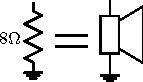
\includegraphics[scale=1.5]{luidspreker}
				\caption{Een luidspreker gedraagt zich ongeveer zoals een weerstand in een elektronisch netwerk.}
				\label{fig:luidspreker}
			\end{figure}

			Wat ons nu interesseert is hoeveel vermogen de weerstand gebruikt, dat gaat een indicatie geven van hoe luid we de muziek kunnen afspelen.
			In de datasheet van de LM386 zit  een belangrijke informatie: de output van de schakeling is een spanningsgolf met maximale amplitude van $3~V$, een een DC-waarde (gemiddelde) gelijk aan $0~V$.
			Dat wilt dus zeggen dat een la bijvoorbeeld kan versterkt worden tot:
			\begin{align}
				V(t) = 3~V \cdot \sin (2\pi \cdot 440~\text{Hz} \cdot t) \\
			\end{align}

			De stroom door de versterker is dan 
				\begin{align}
				I(t) = \frac{3~V}{8~\Omega} \cdot \sin (2\pi \cdot 440~\text{Hz} \cdot t) \\
			\end{align}

			Het vermogen is dan
			\begin{align}
				P(t) = V(t) \cdot I(t) = 1.125~\text{W} \cdot \left( \sin \left(2\pi \cdot 440~\text{Hz} \cdot t\right) \right)^2
			\end{align}

			Omdat muziekgolven veel te snel gaan, hoort de mens alleen de gemiddelde waarde van het vermogen, het gaat niet op en af! 
			Het gemiddelde van een periodieke functie kan uitgerekend worden met een integraal, en dit gaan we doen voor het vermogen. 
			De integraal hangt af van de periode $T$ van de functie, die het inverse is van de frequentie. In ons geval is $T = 1/440Hz \approx 2 ms$.

			\begin{align}
			P_{gemm} &= \frac{1}{T} \int_0^T P(t) dt \\ 
			& = \frac{1}{1/440 \text{Hz}} \int_0^{1/440Hz} 1.125~\text{W} \cdot \left( \sin \left(2\pi \cdot 440~\text{Hz} \cdot t\right) \right)^2 dt
			\end{align}

			\begin{DIY}
				Bereken het gemmiddeld vermogen via de integraal:
				\begin{align*}
				   P_{gemm} \frac{1}{1/440 \text{Hz}} \int_0^{1/440Hz} 1.125~\text{W} \cdot \sin^2 \left(2\pi \cdot 440~\text{Hz} \cdot t\right) dt
				\end{align*}

				Met behulp van de goniometrische formule:
				\begin{align*}
				    \sin^2(\theta) = \frac{1 - \cos(2\theta)}{2}
				 \end{align*}

			\end{DIY}

			Niet alle elektrische energie  wordt omgevormd naar deluidsgolven, veel wordt spijtig genoeg verloren als warmte. Maar zoals je het zelf gaat merken, komt er toch een goed volume uit de luidspreker voor een draagbare speaker.

			Dit be\"eindigt het ontwerp. We hebben gezien dat met enkele wiskundige regels en wat denkwerk, een volledig elektronisch circuit kan ontworpen vanaf simpele componenten. Als je dit een leuke ervaring vond, zijn ingenieursstudies misschien iets voor jou. Je kan online nog veel circuits vinden om zelf te maken! Het circuit moet nu nog alleen gebouwd worden. Op de volgende pagina vind je het volledig circuit. 
	\begin{landscape}
		\section{Overzicht}
				In figuur \ref{fig:volledig_schema} zie je het volledig elektronisch schema van de versterker. Je herkent de twee trappen: de transistorversterker als eerste stap, het IC-circuit als tweede stap. 
				\begin{figure}[htbp]
					\centering
					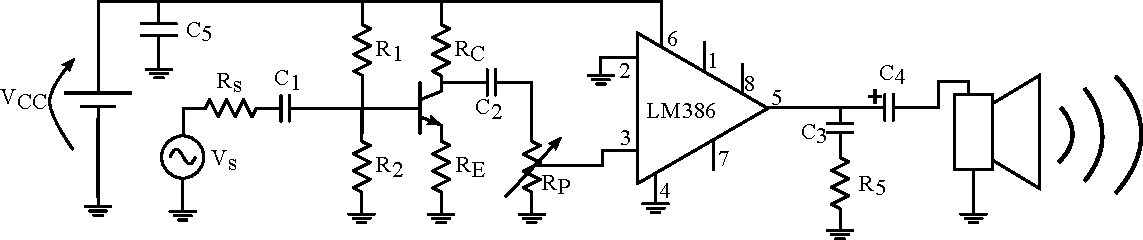
\includegraphics[width=\linewidth]{volledig_schema}
					\caption{Volledig Schema}
					\label{fig:volledig_schema}
				\end{figure}
				$C_1$ en $C_2$ zijn ontkoppelcapaciteiten dienen om DC signalen te blokkeren, $C_5$ werkt als een hulpbatterij.

				Je kan zelf de waarden die je hebt gevonden tijdens het project invullen in het schema. Let wel op dat niet alle weerstandswaarden worden gemaakt, kies waarden die bestaan en die in het labo beschikbaar zijn.
				Als snelle referentie vind je hier voorbeeldwaarden die leiden tot een werkende versterker.

				\begin{center}
					\noindent \fbox{ 
						\parbox{0.8\textwidth}{
							\begin{align*}
								R_1 &= 1~k\Omega & R_2 &= 4.7~k\Omega \\
								R_E &= 100~\Omega & R_C &= 560~\Omega \\
								R_P &= 10~k\Omega & R_5 &= 10~\Omega \\
								R_{LED} &= 680~\Omega
							\end{align*}
						}
					 }
				\end{center}

	\end{landscape}
			\subsection{Printed Circuit Board}
				Voor de e-VUBOX werd een printplaatje gemaakt, waarop je zelf gaat solderen. Figuur \ref{fig:board} kan je zeker helpen om de componenten juist te plaatsen. Let op de richting van de LED, de elektrolytische capaciteit en het IC.
					\begin{figure}[htbp]
					\centering
					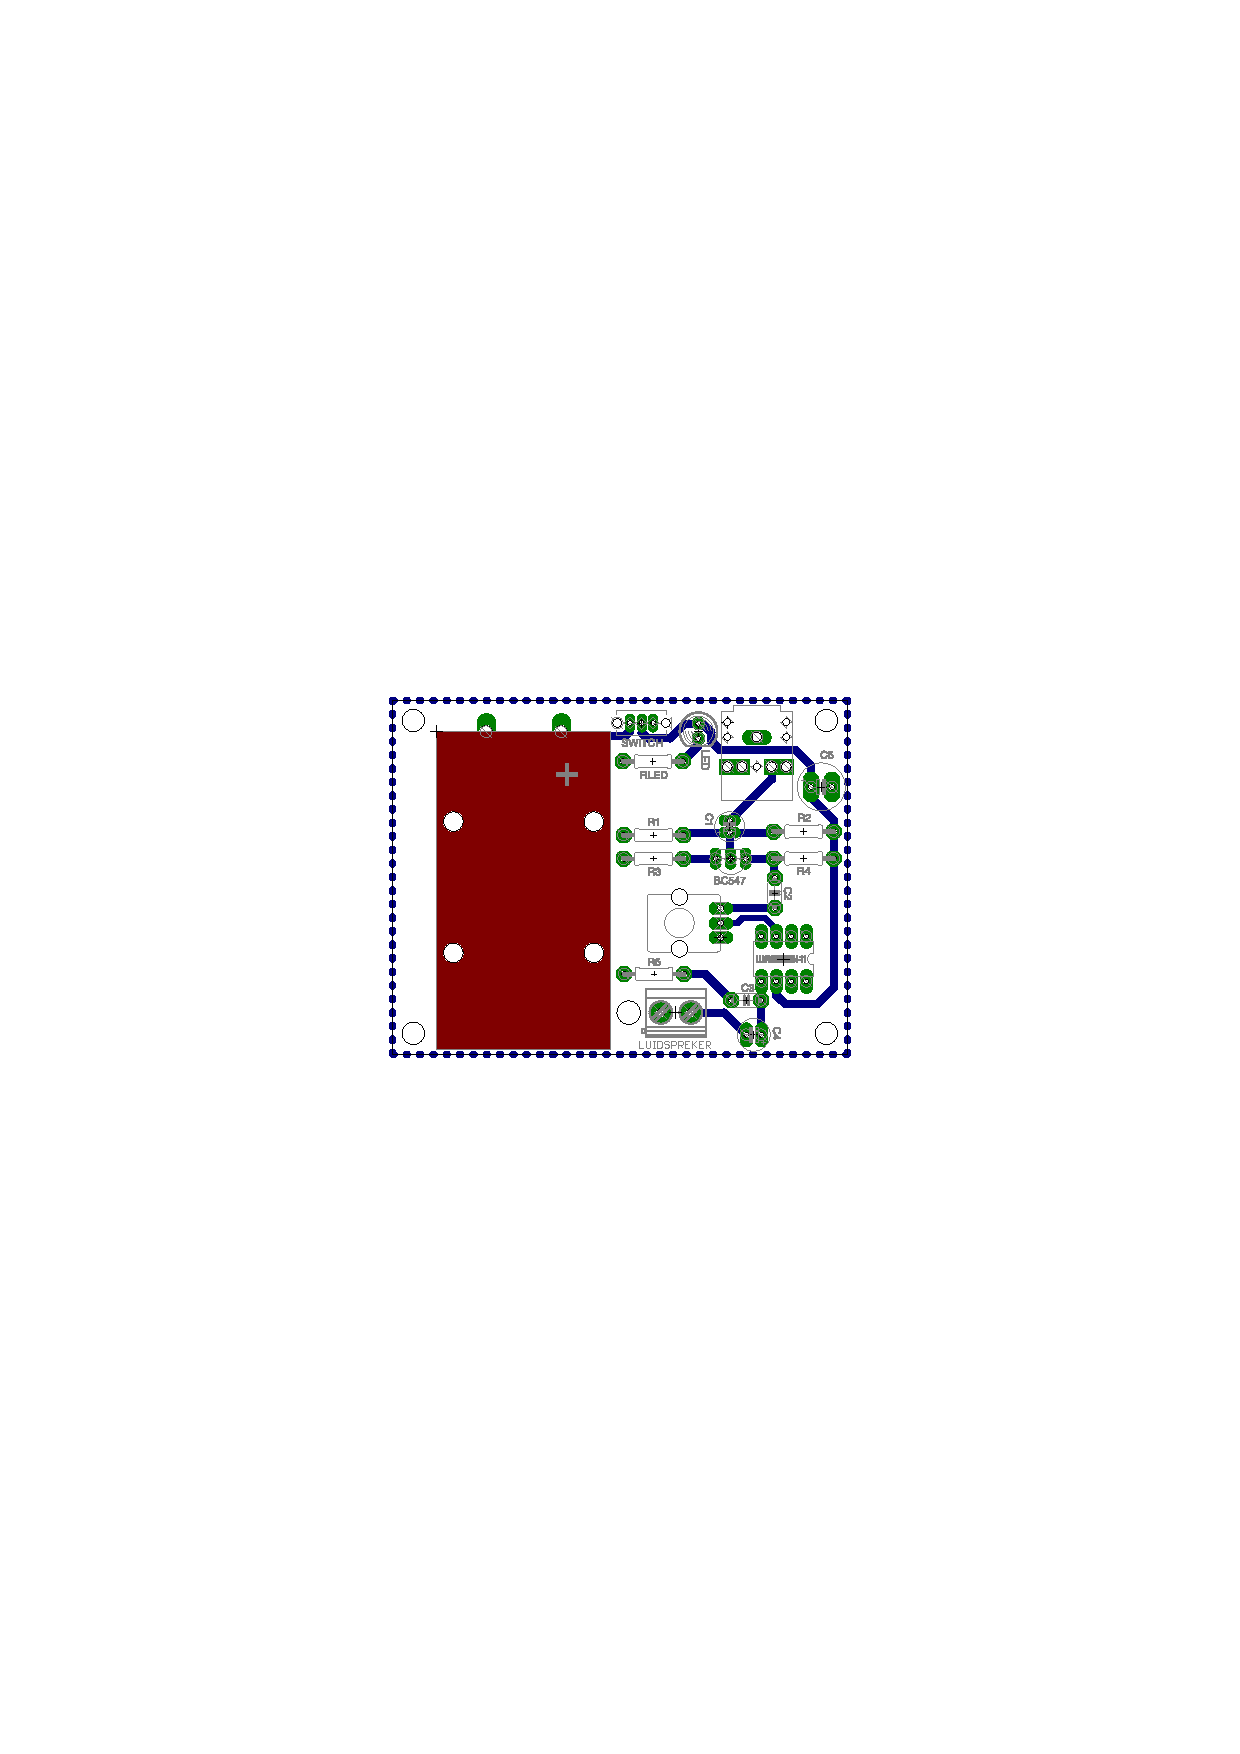
\includegraphics[width=0.95\textwidth]{board}
					\caption{PCB van de e-VUBOX.}
					\label{fig:board}
				\end{figure}
\end{document}